\section{Pilotforsøg}
I dette bilag beskrives pilotforsøgets fremgangsmåde samt, hvilke resultater, der opsamles under udførelsen heraf. 

\subsection{Formål}
Dette pilotforsøg har til formål at kunne præcisere samt optimere kravspecifikationerne i de enkelte blokke, hvorved uklare parametre forventes besvaret. Disse parametre omfatter identificering af støjsignaler, EMG-signalets frekvensområde samt elektrodernes placering. Parametrene vil forsøges besvaret udfra målinger ved udførelse af en squat-øvelse.
Hertil anvendes elektroder og et accelerometer som sensorer. På baggrund af dette opstilles følgende for de enkelte sensorer.  

\subsubsection{EMG-forstærker}
\begin{enumerate}
\item Opsamling af signal fra rectus femoris og biceps femoris
\begin{itemize}
\item Identificering af elektrodernes placering
\item Sammenligning af muskelaktivitet oprejst og i en squat-øvelse 
\end{itemize}
\item Identificering af støjsignaler
\item Identificering af frekvensområde
\item Identificering af gain til mikroprocesserens operationsspænding \fxnote{Finde operationsspænding og angiv den her}
\end{enumerate}

\subsubsection{Accelerometer}
\begin{enumerate}
\item Identificering af knæleddets position siddende i en squat-øvelse
\item Identificering af støjsignaler
\end{enumerate}

\subsection{Materialer} 
\begin{itemize}
\item EMG-forstærker
\item Elektroder \fxnote{hvad for nogle elektroder snakker vi om, husk}
\item Desinfektionsservietter
\item Skraber
\item Accelerometer ADXL335Z
\item Tape
\item Ledninger \fxnote{Er der et navn for ledningen? såsom bananstik}
\item Computer
\item CY8CKIT-042-BLE \fxnote{Opmærksom - er dette den eneste komponent?}
\end{itemize}

\subsection{Metode}
Til forsøget benyttes to EMG-forstærkere og dermed to elektrode sæt, bestående af en positiv-, negativ- samt en referenceelektrode.
For at identificere den bedst mulige elektrodeplacering på musklerne tages der udgangspunkt i den anatomiske afbildning af låret, hvilket ses af \autoref{fig:laarmuskler}.

\begin{figure}[H]
\centering
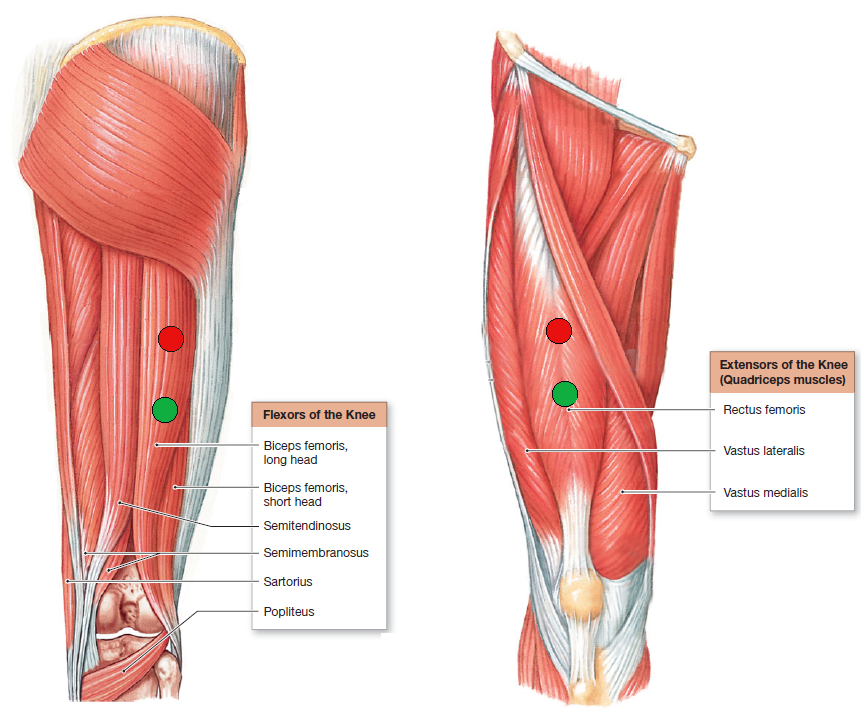
\includegraphics[width=0.5\textwidth]{figures/laarmuskler.png}
\caption{Låret set anteriot og posteriot. Placering af positiv (rød) samt negativ (grøn) elektroder ses på biceps femoris og rectus femoris \citep{martini2012}.}
\label{fig:laarmuskler}
\end{figure}

Elektroderne placeres medialt for både rectus femoris samt biceps femoris for så vidt muligt, at elektroderne forbliver over musklen ved en kontraktion. 

Da der ikke fremgår nogen muskel på den superiore mediale del af tibia, benyttes dette som referencepunkt for EMG-målingen, hvortil der forventes en stabil reference. Placeringen af reference elektroden ses af \autoref{fig:tibia}.

\begin{figure}[H]
\centering
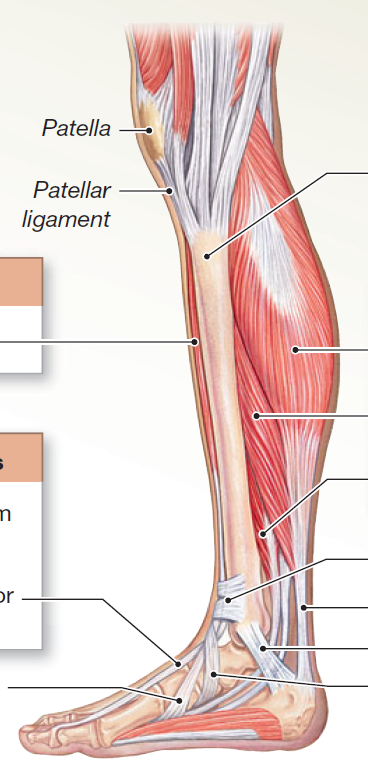
\includegraphics[width=0.2\textwidth]{figures/tibia.png}
\caption{Placering af referenceelektrode på tibia \citep{martini2012}.}
\label{fig:tibia}
\end{figure}

Til identificering af støj fra EMG-forstærkeren fortages der baselinemålinger, som senere analyseres via en frekvensanalyse. Det samme gør sig gældende for identificeringen af EMG-signalets frekvensområde. Dette vil foregå under udførelsen af en squat-øvelse.  

Da mikrokontrolleren benytter en operationsspænding på $XX~V$ ønskes en signalamplitude under operationsspændingen, da dette vil bidrage til en mindre støjpåvirkning. 
%Noget angående signal to noise ratio 

For at simulere den påvirkning som accelerometeret udsættes for og derved identificere det maksimale og minimale outputsignal roteres accelerometeret i en langsom rotation fra $0 - 90^{\circ}$ både til højre og venstre. Herudover måles accelerometerets påvirkning i henholdsvis 0 og 1 g-påvirkning for at identificere accelerometeres påvirkning samt, hvorvidt dette stemmer overens med databladet.


\subsection{Forsøgsopstilling}
Forsøgsopstillingen opstilles i tre dele, hvoraf der først testes med EMG-forstærker, dernæst med accelerometer og til sidst testes de samlet. 

\subsubsection{EMG-forstærker}
\begin{itemize}
\item Identificering af musklerne rectus femoris og biceps femoris 
\item Huden prepereres ved fjernelse af hår og døde hudceller samt desinficering 
\item Elektroderne påsættes
\item Ledningerne påsættes elektroderne
	\begin{itemize}
	\item Elektrodesæt 1: positiv og negativ på rectus femoris
	\item Elektrodesæt 2: positiv og negativ på biceps femoris
	\item Fælles reference på tibia
	\end{itemize} 
\end{itemize}

\subsubsection{Accelerometer}
%Der sørges for, at accelerometeret befinder sig i 0 g-påvirkning ved starten af forsøgets udførelse, hvorved accelerometeret er kaliberet. Dette gøres ved, at middelværdien for målingen trækkes fra, for således at fjerne offset.
\begin{itemize}
\item Accelerometeret placeres lateralt på låret
\item Accelerometeret kobles til måling i y-aksen, således der måles i den vertikale retning
\item Accelerometeret kalibreres
\end{itemize}

\subsection{Fremgangsmåde}
 Forsøgspersonen placeres på et fast punkt fra, hvor følgende øvelser udføres. Forsøget udføres xx antal gange, hvoraf der ud fra målingerne foretages en gennemsnitværdiberegning i en senere frekvensanalyse.

\subsubsection{EMG-forstærker}
\begin{itemize}
\item 10 sekunders baseline måling ved forsøgspersonen står oprejst
\item 10 sekunders måling ved en halv squat-øvelse
	\begin{itemize}
	\item 1 sekunds baseline oprejst
	\item 8 sekunder nedadgående squat 
	\item 1 sekunds baseline i squat-øvelsen
	\end{itemize}
\item 10 sekunders måling ved en fuld squat-øvelse
	\begin{itemize}
	\item 1 sekunds baseline oprejst
	\item 4 sekunder nedadgående squat 
	\item 4 sekunder opadgående squat
	\item 1 sekunds baseline oprejst
	\end{itemize}
\end{itemize}

\subsubsection{Accelerometer}
\begin{itemize}
\item 10 sekunders baseline måling i 0 g-påvirkning (0$^{\circ}$)
\item 10 sekunders baseline måling i 1 g-påvirkning (90$^{\circ}$)
\item 10 sekunders måling ved rotation fra $0-1$ g-påvirkning både til højre og venstre
	\begin{itemize}
	\item 1 sekunds baseline måling i 0 g-påvirkning (0$^{\circ}$
	\item 8 sekunders rotation mod 1 g-påvirkning (90$^{\circ}$)
	\item 1 sekunds baseline måling i 1 g-påvirkning (90$^{\circ}$)
	\end{itemize}
\end{itemize}

